\chapter{Project Management}

\section{Project organisation and tools}

\subsection{GitLab}

GitLab is arguably the best tool out there for managing software projects. It was also important to keep the original code closed source and not expose the CI, and so DoC-hosted GitLab, being protected behind LDAP identification, was well-suited for our use case. At the start of the group project we imported both the existing Voodoo project from a private Github repository, and a fork of the Apache Calcite project. Eight different projects were created or looked at in GitLab over the course of the project duration, five of which are now archived for future reference.

\paragraph{Version control}
Since we are using Git as our version control, we decided to use \textit{feature branches} — when we are, for example, developing a feature or fixing a certain issue, we create a branch specific to that issue (and do not work directly on our main branch). Once our changes are pushed and the CI build is successful (see below), then we can create a merge request into the main branch. These are reviewed by other team members to ensure our code quality, style and correctness is satisfactory, and then merged into the main branch.

\paragraph{Continuous Integration}
Once a team member pushes a commit, we automatically build and test the project to ensure quality and keep master branches healthy (see Fig \ref{fig:calcite-pipeline}). Our CI server is an instance of an Apache CloudStack virtual machine provided by the Department of Computing that is protected behind the Imperial firewall. It allows us to easily hook a device which supports OpenCL. The VM only has Docker installed since we use Docker containers to run the CI. GitLab has a lot of very powerful CI features like caching, which we use to speed up part of the builds, and releases internal artifacts under a fixed job URL which helps with integration tests. Delivering a strong and comprehensive CI was a clear objective of the project, and we discuss it in more detail in subsection \ref{sub:ci-testing}.

\begin{figure}[h]
    \centering
    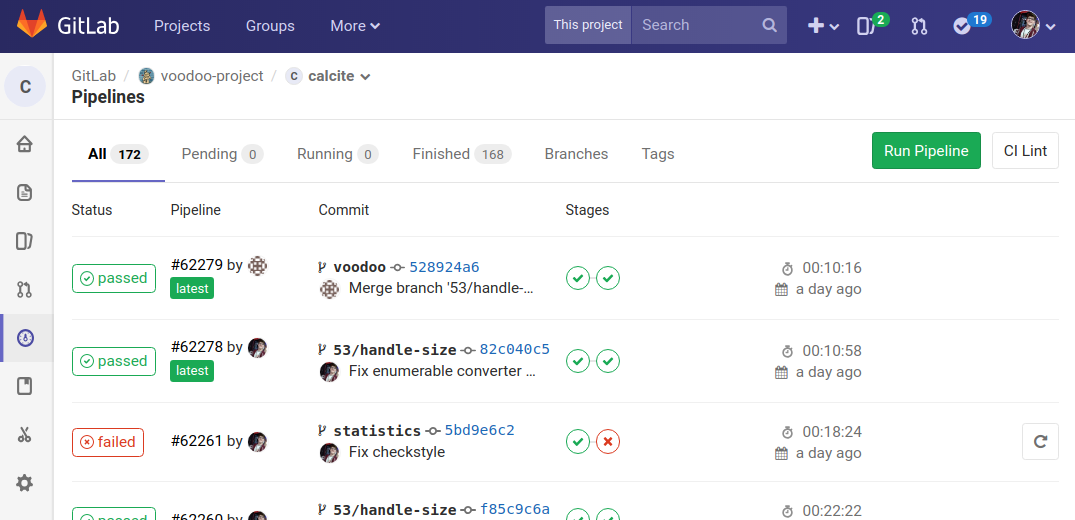
\includegraphics[width=0.98\linewidth, trim={0 0 6cm 7cm}, clip]{project-management/pipeline.png}
    \caption{A list of CI pipelines for the \texttt{calcite} repository}
    \label{fig:calcite-pipeline}
\end{figure}

\paragraph{Issues board structure}
GitLab has a comprehensive issue system, which integrates seamlessly with the merge request and CI interfaces, and also supports several repositories. It also provides a very functional board system (figure \ref{fig:gitlab-issues}) that helped us to gauge at anytime the progress in the checkpoint and to pick up important issues. All issues were divided into the following categories:

\begin{itemize}\itemsep0.2em
    \item \textbf{Backlog}: issues with a low level of priority.
    \item \textbf{To Do}: issues which need to be completed in this iteration, but not being worked on yet.
    \item \textbf{Doing}: issues which some team member(s) is/are currently working on.
    \item \textbf{Closed}: issues which are completed, and the relevant merge requests have been reviewed and merged.
\end{itemize}

\begin{figure}[h]
    \centering
    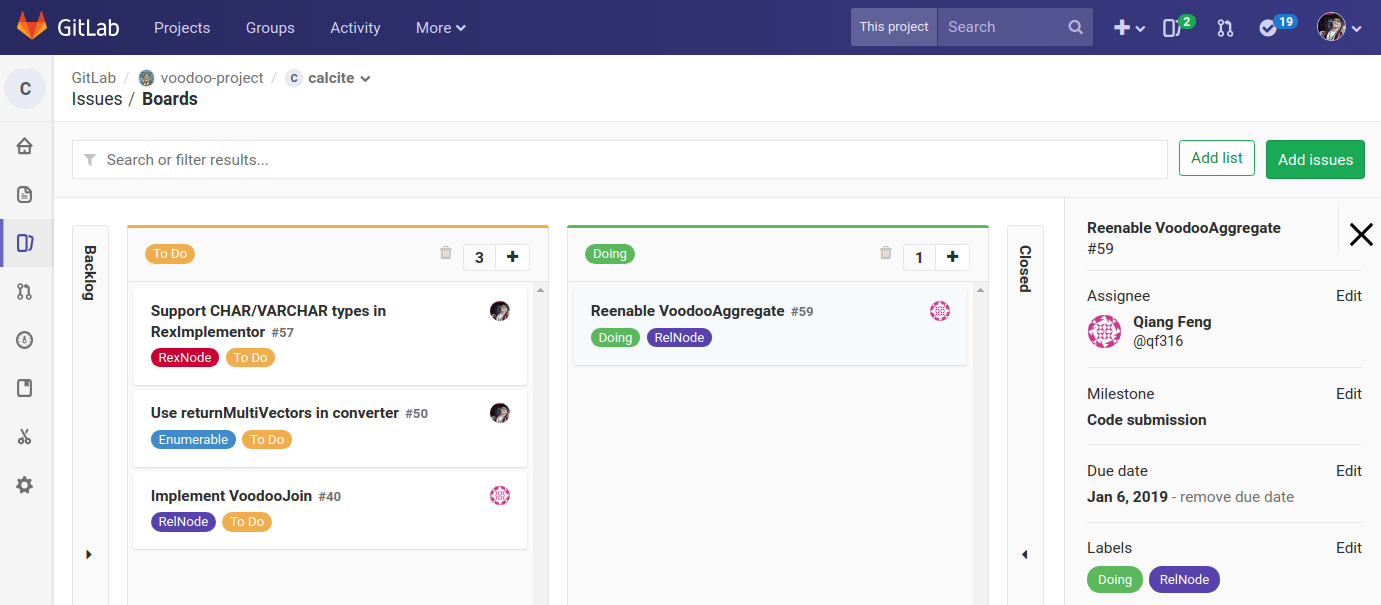
\includegraphics[width=0.98\linewidth, trim={0 0 0 7cm}, clip]{project-management/gitlab-issues.png}
    \caption{Gitlab issues board for our \texttt{calcite} repository}
    \label{fig:gitlab-issues}
\end{figure}

\subsection{Slack}

We decided to use Slack (see Figure \ref{fig:slack}) for online communication since our supervisor was familiar with it.
We kept him updated on the status of the project, and also asked him questions when needed. This turned out to be very useful, especially for the back-end where he could provide details about the existing implementation and explain the Voodoo paper or give us related papers to read.

Slack allows us to have different \emph{channels} so that we can categorise our communications according to which aspect of the project we are discussing. In our case, we have the channels:

\begin{itemize}
    \item \texttt{\#frontend} for communications related to building our Calcite front-end
    \item \texttt{\#codegen} for discussions related to the back-end
    \item \texttt{\#general} to be used for general discussions
    \item \texttt{\#standup} to be used for organising standups for the team
\end{itemize}

For convenience, we used the Gitlab integration within Slack so that we get informed whenever a merge request has been opened or merged, an issue has been opened or closed etc. This information gets displayed in our \texttt{\#gitlab-calcite} and \texttt{\#gitlab-voodoo} channels.

\begin{figure}[h!]
    \centering
    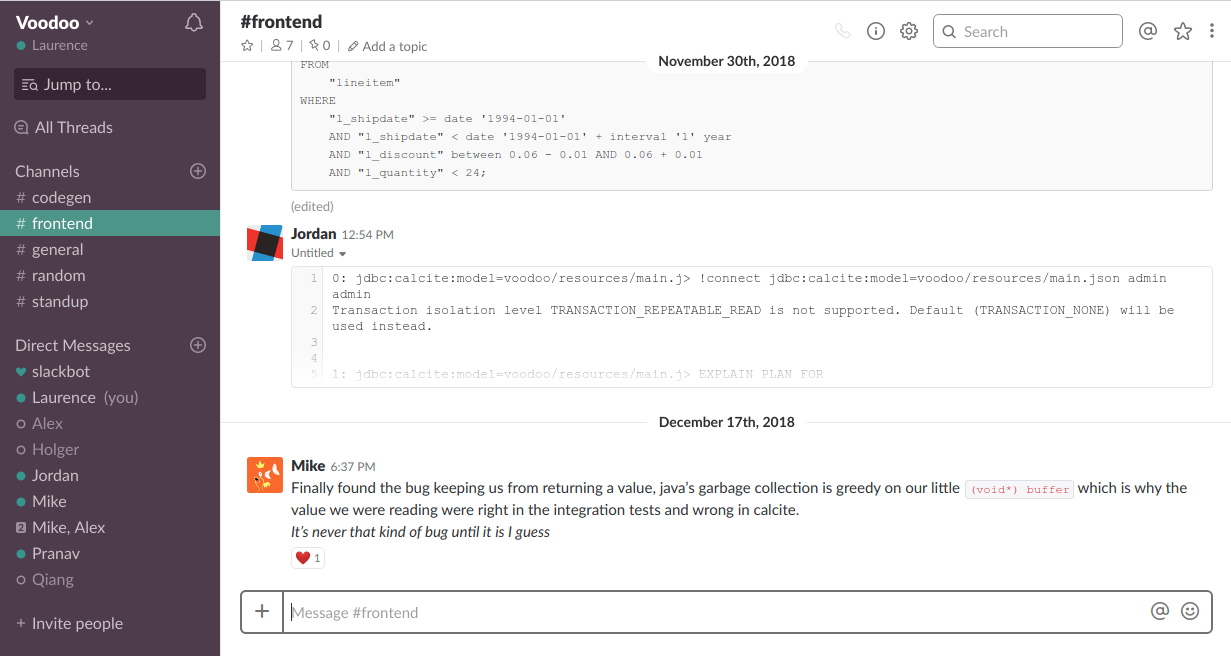
\includegraphics[width=0.9\linewidth]{project-management/slack.png}
    \caption{The \texttt{\#frontend} channel on Slack}
    \label{fig:slack}
\end{figure}

\newpage
\section{Software engineering practices and project planning}

\paragraph{eXtreme Programming} We used eXtreme programming \cite{XP:2013} for this project, a decision which was influenced by the group's previous experience. The various checkpoints and the documentation which we are required to submit fit well into the project schedule. We met with our supervisor on every checkpoint Friday in order to come up with an iteration plan, reflecting on blockers and unfinished issues and figuring out which user stories (TPC-H queries) to integrate into the next plan. We could then write it down and submit it as documentation for each checkpoint, and share it on Slack with our supervisor. We would then use this to manipulate the GitLab issue board, making new issues, closing others, moving them between the different board sections, and making a new milestone to group those issues. At this point, we could begin to discuss how to assign them and how to organise the work for this checkpoint. A lot of independently created issues would appear during the checkpoints, which we would prioritise and work on in due course. These could be bugs that were found, issues about improving some design, or work to do to improve our productivity (and ultimately the productivity of the researchers/users who will work on this project in the future).

\paragraph{Stand-up meetings} To keep all team members updated on the current state of the project we held stand-up meetings. In these meetings, we would discuss the work that had been done and what needed to be done next, and also seek help and form pair programming teams, if there were significant blockers. XP recommends daily meetings, but since this was not a full time project, we adapted daily stand-ups to bi-weekly stand-ups (on Mondays and Wednesdays). Whenever team members were unable to attend stand-ups in person, we would still continue to hold standups through Messenger video calls.

\subsection{Project timeline}

We pivoted from another project in the middle of checkpoint 1. At this time, we had an initial meeting with our supervisor, where we discussed the goals for the project. These formed the basis of our \emph{release plan}. We were also given access to an existing codebase and the research paper for Voodoo. Below, we summarise main goals of the iteration plan:

\paragraph{Checkpoint 1} 
After investigating and gaining familiarity with the existing Voodoo codebase and its concept, come up with a AST to represent the TPC-H query 6 code — this was code that we had to generate from the existing codebase after making all the adjustments necessary to be able to compile and run it on our systems.

\paragraph{Checkpoint 2}
Generate Voodoo vector algebra for TPC-H query 6 in Java using the existing \texttt{Printer} implementation after forming a Calcite plan. Investigate the best technology to generate the AST from Checkpoint 1, and use it to assemble the AST from checkpoint 1.

\paragraph{Checkpoint 3}
Generate Voodoo vector algebra for TPC-H queries 1 and 19, and have query 6 running using the \texttt{ClangAst} back-end, generating and running the right OpenCL code.

\paragraph{Checkpoint 4}
Generate and retrieve results for TPC-H queries 1, 6 and 19 by using a JDBC connection to Calcite by implementing an adapter, generate correct Voodoo and OpenCL code for them, and run OpenCL on the front-end data.

We implemented \emph{acceptance tests} from those objectives. For example automation of installation and CI work for checkpoint 1, use the printer implementation to check the correct output of the front-end in checkpoint 2, check the value of the result vector from a Voodoo program in checkpoint 3 and checking the value of a vector from an SQL query in checkpoint 4.

We expected there to be alterations to these objectives due to technical challenges we might face. We learned to plan according to our \emph{project velocity} with our supervisor, even using \emph{planning poker} as to better share our ideas on the time particular tasks would take. Communicating effectively with our supervisor during the iteration meetings was probably the biggest management challenge but is something we have consistently become better at.

The team naturaly split into specialised groups due to the complexity and depth of the front-end and back-end code-bases: it required a fairly significant time investment to fully understand each component, and so we thought it would be unreasonable to expect all team members to be able to work on all components. As such, \textbf{Qiang} and \textbf{Jordan} developed the Calcite front-end, \textbf{Laurence} and \textbf{Alex} worked on the Voodoo back-end, and \textbf{Mayeul} and \textbf{Pranav} managed the good integration of the two sides, and worked on issues that required knowledge of both the front-end and back-end.

A point to note is that due to the nature of the project, the first few tasks were long and required multiple team members working on a single task. However, as we improved our knowledge of the existing codebase and, more importantly, improved the project structure, it was then possible to break down objectives into smaller tasks that each individual could take ownership of - hence enabling us to iterate more in a checkpoint. This is demonstrated by the increase in frequency and reduction in size of merge requests as the project progressed.
